\section{PROOFS}
\label{app:proofs}

Throughout, $w_i(\rho)=\lambda_i/(\lambda_i+\rho)$, and $M$ matrices are symmetric.

\paragraph{Proof of \Cref{thm:identity}.}
Write $a=\phi_A(x)$, $b=\phi_B(x)$, $P=M_A$, $Q=M_B$. For a zero-mean Gaussian vector, Isserlis' theorem \citep{isserlis1918} gives
$\E[a_ia_jb_kb_l]=(\Sigma_A)_{ij}(\Sigma_B)_{kl}+(\Sigma_{AB})_{ik}(\Sigma_{AB})_{jl}+(\Sigma_{AB})_{il}(\Sigma_{AB})_{jk}$.
Contracting with $P_{ij}Q_{kl}$ and using the symmetry of $P,Q$,
\[
\E[a^\top Pa\; b^\top Qb]=\tr(P\Sigma_A)\tr(Q\Sigma_B)+2\tr(P\Sigma_{AB}Q\Sigma_{BA}).
\]
Since $\E[a^\top Pa]=\tr(P\Sigma_A)$, $\mathrm{Cov}(a^\top Pa,b^\top Qb)=2\tr(P\Sigma_{AB}Q\Sigma_{BA})$. Setting $b=a$, $Q=P$ gives $\mathrm{Var}(a^\top Pa)=2\tr((P\Sigma_A)^2)$, and likewise for $b$. Dividing gives $S(M_A,M_B)$. For $u_A,u_B$ take $M_A=(\Sigma_A+\rho_AI)^{-1}$, $M_B=(\Sigma_B+\rho_BI)^{-1}$. \hfill$\square$

\paragraph{Proof of \Cref{prop:limits}.}
(i) As $\rho\to\infty$, $\rho M_A\to I$ and $\rho M_B\to I$. Multiplying numerator and both factors of the denominator by $\rho^2$, the numerator tends to $\tr(\Sigma_{AB}\Sigma_{BA})=\|\Sigma_{AB}\|_F^2$ and the denominator to $\sqrt{\tr(\Sigma_A^2)\tr(\Sigma_B^2)}=\|\Sigma_A\|_F\|\Sigma_B\|_F$.
(ii) As $\rho\to0$, $M_A\to\Sigma_A^{-1}$; the numerator tends to $\tr(\Sigma_A^{-1}\Sigma_{AB}\Sigma_B^{-1}\Sigma_{BA})=\|\Sigma_A^{-1/2}\Sigma_{AB}\Sigma_B^{-1/2}\|_F^2=\sum_jr_j^2$, and $\tr((\Sigma_A^{-1}\Sigma_A)^2)=d_A$. The limit is therefore $\sum_jr_j^2/\sqrt{d_Ad_B}$, which equals the mean squared canonical correlation only when $d_A=d_B$. \hfill$\square$

\paragraph{Proof of \Cref{cor:neither}.}
$\Sigma_{AB}=\mathrm{diag}(\lambda_sI_k,0)$ and $M_A=\mathrm{diag}((\lambda_s+\rho)^{-1}I_k,(\lambda_p+\rho)^{-1}I_m)$, so the numerator of $\Srho$ is $kw_s^2$ and $\tr((M_A\Sigma_A)^2)=kw_s^2+mw_p^2$; CKA follows the same way with $\lambda$ in place of $w$.
\emph{High CKA, low agreement:} take $\rho\le\lambda_p$ (so $w_p\ge\frac12$, $w_s\le1$) and $m\ge4k/\epsilon$; then $\corr\le k/(k+m/4)\le\epsilon$. Then take $\lambda_p/\lambda_s\le\sqrt{\epsilon k/m}$, so $\cka=1/(1+(m/k)(\lambda_p/\lambda_s)^2)\ge1/(1+\epsilon)\ge1-\epsilon$.
\emph{Low CKA, high agreement:} take $\rho\le\lambda_s$ (so $w_s\ge\frac12$) and $k\ge4m/\epsilon$; then $\corr=1/(1+mw_p^2/(kw_s^2))\ge1-4m/k\ge1-\epsilon$. Then take $\lambda_p/\lambda_s\ge\sqrt{k/(m\epsilon)}$, so $\cka\le k\lambda_s^2/(m\lambda_p^2)\le\epsilon$. \hfill$\square$

\paragraph{Proof of \Cref{prop:scale}.}
CKA and cosine similarities are invariant to $\phi\mapsto cQ\phi$. For the variance,
$v(cQ\Phi,cQx;\lambda)=\sigma^2c^2x^\top Q^\top(c^2Q\Phi^\top\Phi Q^\top+\lambda I)^{-1}Qx=\sigma^2x^\top(\Phi^\top\Phi+(\lambda/c^2)I)^{-1}x$.
So the transformed head is the original head with prior strength $\rho/c^2$. Apply \Cref{thm:identity} to the same features with $M_A=(\Sigma+\rho c^{-2}I)^{-1}$, $M_B=(\Sigma+\rho I)^{-1}$, $\Sigma_{AB}=\Sigma$: the numerator is $\sum_iw_i(\rho/c^2)w_i(\rho)$ and the denominators are $\sum_iw_i(\cdot)^2$. By Cauchy--Schwarz the ratio equals one iff $w_i(\rho)/w_i(\rho/c^2)=(\lambda_i+\rho/c^2)/(\lambda_i+\rho)$ is constant over the support, i.e.\ iff the nonzero $\lambda_i$ are equal (for $c\ne1$). \hfill$\square$

\paragraph{Proof of \Cref{prop:tail}.}
With $T_s=U\,\mathrm{diag}(s_i)U^\top$ ($s_i=s$ on $\mathcal T$, $1$ otherwise), $\E[\phi(T_s\phi)^\top]=U\Lambda\,\mathrm{diag}(s_i)U^\top$ and $\mathrm{Cov}(T_s\phi)=U\Lambda\,\mathrm{diag}(s_i^2)U^\top$. Hence
$\cka=\sum\lambda_i^2s_i^2/\sqrt{\sum\lambda_i^2\sum\lambda_i^2s_i^4}=(1+s^2\eta)/\sqrt{(1+\eta)(1+s^4\eta)}$.
Moreover $1-\cka^2=\eta(s^2-1)^2/((1+\eta)(1+s^4\eta))\le\eta(s^2-1)^2$, and $\cka\ge\cka^2$ since $\cka\le1$. The transformed eigenvalues are $s^2\lambda_i$ on $\mathcal T$, and $s^2\lambda_i/(s^2\lambda_i+\rho)=w_i(\rho/s^2)$. \hfill$\square$

\paragraph{Proof of \Cref{lem:deff}.}
$\sum_iv(x_i)=\sigma^2\tr(\Phi(\Phi^\top\Phi+\lambda I)^{-1}\Phi^\top)=\sigma^2\sum_ig_i/(g_i+\lambda)$ with $g_i=n\hat\lambda_i$ the eigenvalues of $\Phi^\top\Phi$; divide by $n$ and use $\lambda/n=\rho$. \hfill$\square$

\paragraph{Proof of \Cref{cor:same}.} \Cref{thm:identity} with $\Sigma_A=\Sigma_B=\Sigma_{AB}=\Sigma$, $M_j=(\Sigma+\rho_jI)^{-1}$. \hfill$\square$

\paragraph{Proof of \Cref{lem:boot}.}
With $y=\Phi w+\varepsilon$, $\mathrm{Cov}(\varepsilon)=\sigma^2I$ and $\hat w=A^{-1}\Phi^\top y$, $\mathrm{Cov}_\varepsilon(\hat w)=\sigma^2A^{-1}\Phi^\top\Phi A^{-1}=\sigma^2A^{-1}GA^{-1}$. In the eigenbasis of $G$ this is $\sigma^2g_i/(g_i+\lambda)^2$, against the posterior $\sigma^2/(g_i+\lambda)$. Residual resampling estimates this noise covariance as $n\to\infty$. The EU score is $\phi^\top\mathrm{Cov}(\hat w)\phi=\frac{\sigma^2}{n}\phi^\top(\hat\Sigma+\rho)^{-1}\hat\Sigma(\hat\Sigma+\rho)^{-1}\phi$, so in \Cref{thm:identity} $M\Sigma$ has eigenvalues $w_i^2$ and the direction weights are $w_i^4$. \hfill$\square$

\paragraph{Proof of \Cref{prop:resolvent}.}
$G$ and $(G+s^2I)^{-1}$ commute, so $\mathrm P(G)=G(G+s^2I)^{-1}[(G+s^2I)-G]=s^2(I-s^2(G+s^2I)^{-1})$. Hence $\mathrm P(K)-\mathrm P(L)=s^4[(L+s^2I)^{-1}-(K+s^2I)^{-1}]=s^4(K+s^2I)^{-1}(K-L)(L+s^2I)^{-1}$, and $\|(G+s^2I)^{-1}\|_{\mathrm{op}}\le s^{-2}$ for $G\succeq0$. \hfill$\square$

\paragraph{The bound fails for unobserved points.}
For $Z=\mathcal T\cup\mathcal E$ with only $\mathcal T$ observed, $\mathrm P(G)=G-G_{Z\mathcal T}(G_{\mathcal T\mathcal T}+s^2I)^{-1}G_{\mathcal TZ}$. In 3000 random trials (feature dimension 1--11, $|\mathcal T|\in[3,30)$, $|\mathcal E|\in[1,20)$, $s^2\in[10^{-2},10]$) the ratio $\|\mathrm P(K)-\mathrm P(L)\|_{\mathrm{op}}/\|K-L\|_{\mathrm{op}}$ reached \ResolventWorst{}, so no constant-one bound holds there.

\section{EXPERIMENTAL DETAILS}
\label{app:details}

\paragraph{Pre-registration.} The \texttt{PREREG} dictionary (claims, falsifiers, gate) was frozen before any real-data computation; its SHA-256 is \texttt{\PreregHashFull} (file \texttt{PREREG\_FROZEN.txt} in the supplementary code, frozen 2026-10-02 before any real-data computation; no external registry was used, so the hash certifies content, not time). The frozen falsifiers for E2-b (``AU degrades as much as EU'') and S (``no better than CKA'') carried no numeric threshold; the operational rules in \Cref{tab:prereg} were fixed by us when computing them and are therefore post hoc. Analyses not in the pre-registration (the $\Srho$ evaluation at $\rho\to0$, the $\deff$-versus-participation-ratio contrast, the exploratory E4 variant, and all post-review analyses in \Cref{app:revision}) are exploratory.

\paragraph{Features.} Taps at relative depths $0.5,0.75,1$ of the flattened block list; mean over patch tokens excluding prefix tokens (ViTs) or spatial mean (ConvNeXt) of the raw block output; fp16 cache; bicubic upsampling $32\to224$ with each encoder's own normalisation. DINOv2 uses \texttt{img\_size=224} with interpolated position embeddings.

\paragraph{Heads.} Softmax regression, objective $\sum_iw_i\,\mathrm{CE}_i/\sum_iw_i+\frac{\mathrm{wd}}2\|W\|^2$, full-batch L-BFGS (strong Wolfe, $\le200$ iterations), all $M$ members trained in one tensor; agreement with scikit-learn's optimum to $5\times10^{-4}$ in probability. Weight decay grid $\{10^{-5},\dots,10^{-1}\}$, chosen by validation NLL on a fixed 10k split of the training set with hard labels. Poisson(1) bootstrap weights. EU summaries: summed $5$--$95\%$ quantile width over classes and mutual information; AU: mean member entropy. Laplace: class-block-diagonal GGN at the MAP of member 0 with prior precision $n\cdot\mathrm{wd}$, 100 Monte Carlo logit samples. Closed-form EU: $u(x)=\phi^\top(\hat\Sigma+\rho I)^{-1}\phi$ with $\rho=\mathrm{wd}$.

\paragraph{Ensemble size.} \MChoice

\paragraph{Statistics.} Item-level Spearman; partial Spearman on ranks residualised on both models' confidence (max mean probability) and human plug-in entropy; stratified Spearman within human-entropy deciles. CIFAR-10H ceiling: split votes into halves without replacement (multivariate hypergeometric), Spearman between half entropies, Spearman--Brown corrected, 50 repetitions.

\paragraph{Compute.} One Apple M2 Pro laptop (16\,GB), PyTorch MPS for feature extraction (68--113 images/s) and CPU float32/float64 for heads and linear algebra.

\paragraph{Licences.} CIFAR-10H: CC BY-NC-SA 4.0. Model weights via \texttt{timm} and \texttt{open\_clip} under their respective licences.

\section{POST-REVIEW ANALYSES}
\label{app:revision}
All analyses in this section were added after an internal round of review and are exploratory.
\paragraph{Leave-one-encoder-out sensitivity.} The 30 encoder pairs share encoders, so they are not independent, and with five encoders a cluster bootstrap is degenerate (few distinct resamples, many with fewer than three pairs). We therefore recompute every correlation on the five subsets that leave out one encoder (18 pairs each) and report the range and the number of subsets in which a difference is positive. These ranges describe sensitivity; they are not confidence intervals. An earlier draft reported percentile cluster-bootstrap intervals, which we withdrew for this reason.
\paragraph{Reliability and redraws.} For each encoder (final depth, selected weight decay, $M=50$) we draw three independent 10\% subsets and three independent splits into halves; every head is fitted twice with different Poisson weights. A pair's corrected agreement is its partial agreement divided by $\sqrt{r_{xx}r_{yy}}$, where $r_{xx}$ is the partial agreement between the two replicates of head $x$. The re-test ensembles use seeds 0 and 1 of the full-data head. In the E2b re-tuning, the selected weight decays lie on the boundaries of the searched grid for $c=0.1$ and $c=10$, so the re-tuned values are bounds rather than interior optima.
\paragraph{Weight-decay sweep.} All 15 encoder--depth heads are refitted with $M=20$ at a common weight decay $\rho\in\{10^{-3},10^{-2},10^{-1},1\}$ (no validation selection), and agreement and indices are recomputed for the 30 pairs. Training-only $\Srho$ uses the same 10k training subset without test inputs.

\section{ADDITIONAL RESULTS}
\label{app:results}
\begin{figure}[h]
\centering
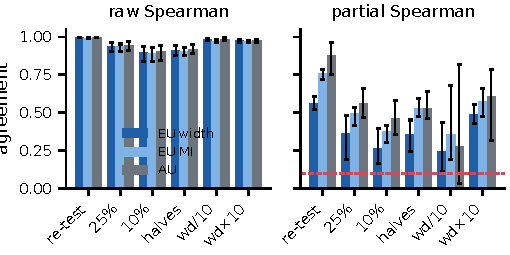
\includegraphics[width=0.6\textwidth]{figures/fig_e2.pdf}
\caption{E2: agreement between heads on identical features, mean over five encoders (bars: min--max). Right: partial Spearman controlling for both heads' confidence and human entropy; the dashed line is the mean partial EU agreement between \emph{different} encoders at the final depth.}
\label{fig:e2}
\end{figure}
\begin{figure}[h]
\centering
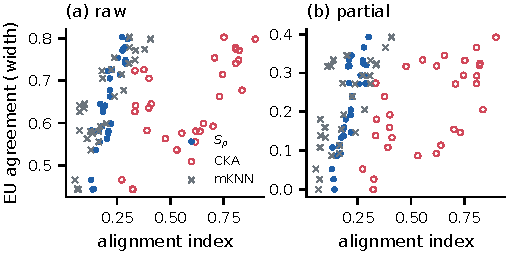
\includegraphics[width=0.6\textwidth]{figures/fig_real.pdf}
\caption{Across 30 encoder pairs (5 encoders, 3 depths): item-level bootstrap EU agreement, raw \textbf{(a)} and partial \textbf{(b)}, against $\Srho$ at the heads' $\rho$ (filled), CKA (open) and mutual $k$-NN (crosses).}
\label{fig:real}
\end{figure}

\begin{table}[h]
\centering
\caption{E2 per encoder: Spearman (partial) agreement for EU width, mutual information and AU, and model AU versus human entropy (fraction of ceiling).}
\small
\begin{tabular}{llccc}
\toprule
encoder & pair & EU width & EU MI & AU \\
\midrule
DINOv2-B & re-test floor & 1.00 (0.61) & 0.99 (0.78) & 1.00 \\
DINOv2-B & 25\% vs 100\% data & 0.96 (0.48) & 0.95 (0.54) & 0.97 \\
DINOv2-B & 10\% vs 100\% data & 0.94 (0.40) & 0.93 (0.42) & 0.94 \\
DINOv2-B & disjoint halves & 0.94 (0.45) & 0.93 (0.55) & 0.95 \\
DINOv2-B & wd $\div10$ & 0.99 (0.28) & 0.96 (0.19) & 0.99 \\
DINOv2-B & wd $\times10$ & 0.98 (0.55) & 0.98 (0.53) & 0.98 \\
DINOv2-B & AU vs human & \multicolumn{3}{c}{0.36 (0.43 of $\sqrt{\text{ceiling}}$); test acc. 0.98} \\ \midrule
CLIP-B/16 & re-test floor & 1.00 (0.52) & 0.99 (0.73) & 1.00 \\
CLIP-B/16 & 25\% vs 100\% data & 0.95 (0.33) & 0.94 (0.50) & 0.95 \\
CLIP-B/16 & 10\% vs 100\% data & 0.90 (0.21) & 0.89 (0.39) & 0.90 \\
CLIP-B/16 & disjoint halves & 0.91 (0.30) & 0.91 (0.52) & 0.92 \\
CLIP-B/16 & wd $\div10$ & 0.98 (0.11) & 0.97 (0.35) & 0.97 \\
CLIP-B/16 & wd $\times10$ & 0.97 (0.45) & 0.96 (0.58) & 0.96 \\
CLIP-B/16 & AU vs human & \multicolumn{3}{c}{0.43 (0.51 of $\sqrt{\text{ceiling}}$); test acc. 0.95} \\ \midrule
ViT-B/16 sup. & re-test floor & 1.00 (0.55) & 0.99 (0.72) & 1.00 \\
ViT-B/16 sup. & 25\% vs 100\% data & 0.95 (0.43) & 0.95 (0.49) & 0.96 \\
ViT-B/16 sup. & 10\% vs 100\% data & 0.93 (0.25) & 0.92 (0.30) & 0.93 \\
ViT-B/16 sup. & disjoint halves & 0.94 (0.39) & 0.93 (0.48) & 0.95 \\
ViT-B/16 sup. & wd $\div10$ & 0.99 (0.28) & 0.97 (0.21) & 0.99 \\
ViT-B/16 sup. & wd $\times10$ & 0.98 (0.43) & 0.97 (0.48) & 0.98 \\
ViT-B/16 sup. & AU vs human & \multicolumn{3}{c}{0.35 (0.42 of $\sqrt{\text{ceiling}}$); test acc. 0.98} \\ \midrule
ConvNeXt-S & re-test floor & 1.00 (0.55) & 0.99 (0.78) & 1.00 \\
ConvNeXt-S & 25\% vs 100\% data & 0.93 (0.39) & 0.93 (0.54) & 0.94 \\
ConvNeXt-S & 10\% vs 100\% data & 0.88 (0.28) & 0.88 (0.41) & 0.89 \\
ConvNeXt-S & disjoint halves & 0.88 (0.40) & 0.88 (0.59) & 0.89 \\
ConvNeXt-S & wd $\div10$ & 0.98 (0.12) & 0.97 (0.35) & 0.98 \\
ConvNeXt-S & wd $\times10$ & 0.97 (0.50) & 0.97 (0.63) & 0.97 \\
ConvNeXt-S & AU vs human & \multicolumn{3}{c}{0.34 (0.40 of $\sqrt{\text{ceiling}}$); test acc. 0.97} \\ \midrule
MAE-B/16 & re-test floor & 0.99 (0.58) & 0.99 (0.76) & 1.00 \\
MAE-B/16 & 25\% vs 100\% data & 0.90 (0.19) & 0.90 (0.41) & 0.91 \\
MAE-B/16 & 10\% vs 100\% data & 0.84 (0.17) & 0.84 (0.35) & 0.85 \\
MAE-B/16 & disjoint halves & 0.88 (0.24) & 0.87 (0.48) & 0.89 \\
MAE-B/16 & wd $\div10$ & 0.99 (0.44) & 0.98 (0.68) & 0.99 \\
MAE-B/16 & wd $\times10$ & 0.97 (0.52) & 0.97 (0.66) & 0.98 \\
MAE-B/16 & AU vs human & \multicolumn{3}{c}{0.38 (0.46 of $\sqrt{\text{ceiling}}$); test acc. 0.90} \\
\bottomrule
\end{tabular}
\end{table}
\begin{table}[h]
\centering
\caption{Across 30 encoder pairs: Spearman correlation between alignment indices and item-level agreement of EU (and AU), all columns.}
\label{tab:srhofull}
\small
\begin{tabular}{lccccc}
\toprule
index & width & width partial & MI & BLR & AU \\
\midrule
CKA & 0.66 & 0.64 & 0.67 & 0.76 & 0.68 \\
mutual $k$-NN & 0.85 & 0.72 & 0.86 & 0.90 & 0.86 \\
linear predictivity & 0.41 & 0.83 & 0.44 & 0.56 & 0.53 \\
$S_{\rho\to0}$ & 0.88 & 0.83 & 0.90 & 0.93 & 0.93 \\
$S_\rho$ (head's $\rho$) & 0.87 & 0.83 & 0.89 & 0.92 & 0.92 \\
\bottomrule
\end{tabular}
\end{table}
